\chapter{Text analysis with deep learning}

\section{\ac{nlp}}
\ac{nlp} is the field of designing methods that take as input or
produce as output natural language data. Natural language is
ambiguous and variable, for instance the sentence ``i saw a woman on a
hill with a binocular'' can means that I had a binocular and with
those I saw a
woman on a hill, or that a woman was on a hill using the
binocular. This ambiguity can also be the source of problems in
specific context as the medical text, where specific countermeasures
can be adopted \cite{zhao_clinical_2019,codish2005model}.

Language is
\emph{symbolic} and \emph{discrete}, the relationship between different words,
i.e. symbols, can not be inferred from the symbols
themselves. It is possible to easily compare concepts that have a
continuous representation, e.g. two different colors in an image,
while it cannot be done easily with words without using large lookup
table or advanced methods. Language is also \emph{compositional},
letters form words, and words form sentences. Language is also
\emph{sparse}, the way in which words can be combined to form meanings
is practically infinite.

\section{\ac{ann} in \ac{nlp}}
\ac{ml} approaches are characterized by learning to make predictions
based on past observations. \ac{ann} approaches work by learning not
only to predict, but also to correctly represent data. A common
component of \ac{ann} applied to \ac{nlp} is the embedding layer,
i.e. a mapping from discrete symbols to continuous vectors in a
relatively low dimensional space. This representation allows to
transform the isolated symbols into mathematical objects that can be
operated on.

The principal model that is used in \ac{nlp} are \ac{rnn}. They are
capable of producing a vector that summarize the entire input
sequence. They allow abandoning the \emph{markov} assumption that was
prevalent in \ac{nlp} for decades, and designing models that can
condition on entire sentences or documents. This capability leads to
impressive gains in \emph{language-modeling}, the task of predicting
the probability of the next word in a sequence.

\subsection{Features}
The mapping from textual data to real valued vector that can be used
as input for \ac{ann} models, is called \emph{features extraction}.

When the focus entity is a word outside of a context, the main source
of information is the letters. We can look at \emph{lemma},
i.e. dictionary entry of the word, e.g. words such as ``booking'',
``booked'', ``books'' to their common lemma ``book''. This mapping is
usually performed using lemma lexicons or morphological analyzers. It
is a linguistically defined process and may not work well for forms
that are not in the lexicon or for mispelling. A coarser process is
called \emph{stemming}, it maps words to shorter words that are
not necessarily grammatically valid. E.g. ``picture'', ``pictures'',
and ``pictured'' will be stemmed to ``pictur''. \emph{Lexical
  resources} are dictionary that are meant to be accessed by machine
rather than by humans. They typically contain information about words,
e.g. there are lexicons that map inflected word forms to their
possible morphological analyses, telling that a certain word may be a
singular masculine noun or a past-perfect verb.

When the focus entity is text, i.e. sentences, paragraphs documents,
the features are the count and the order of the letters and words
within the text. \emph{Bag of words} is a very common feature
extraction procedure. We look at the histogram of the words within the
text. We can compute quantities that are directly derived from
the words and the letters such as the length of the sentence. We can
also integrate statistics based on external information. When using
bag of words, it is common to use \ac{tfidf} weighting
\cite{manning_introduction_2008}. A word $w$ in a document $d$ that is
part of a large corpus $D$ of documents is represented by:
\begin{equation*}
  \frac{\#_d(w)}{\sum_{w'\in d}\#_d(w')}\cdot\log\frac{|D|}{|d\in
    D:w\in d|},
\end{equation*}
where $\#_d(w)$ is the number of times that $w$ appears in
$d$. Besides words, one may also look at consecutive pairs or triplets
of words. These are called \emph{ngrams}. A bag of ngrams
representation is much more informative than a bag of words.

When considering a word within a sentence or a document, the features
of a word are its position within the sentence and the words or
letters surrounding it. It is common to focus on the immediate context
of a word by considering a \emph{window} surrounding it (with typical
values of 2, 5, and 10 words to each side). We may also be interested
in the absolute position of a word inside a sentence, having features
such as ``the word is the 5th in the sentence'' or ``the word appear
within the first 10 of the sentence''.

When considering more than a word within a context, we can also look
at the text \emph{distance} between them or the identities of the
words that appear between them.

Sentences in natural language have structures beyond the linear order
of their words. The structure is not directly observable and is
referred to as \emph{syntax}. While it is not observable it can be
inferred from the sentence. Specialized systems exist for the
prediction of parts of speech, syntactic trees, semantic roles,
discourse relations, and other linguistic properties. These prediction
often serve as good features for classification problems.

Different features can also be combined together. Instead of combining
them manually, we can provide a set of core features to an \ac{ann}
model and rely on the training procedure to pick up important
combinations of them.
Core features can also be learned by \ac{ann}, but enough data is
needed. The distributional hypothesis of language states that the
meaning of a word can be inferred from the contexts in which it is
used. By observing co-occurrence patterns of words across a large body
of text, it is possible to infer that a word is similar to another
word. Many algorithms were derived to make use of this property. They
can be categorized into clustering-based methods, with assign similar
words to the same cluster and represent each word by its cluster
membership \cite{miller2004name}, and embedding-based methods which
represent each word as a 
vector such that similar words (with similar distribution) have
similar vectors \cite{pennington_glove:_2014,mikolov_linguistic_2013}.

\section{Text classification}
\label{sec-baselines}
The classic approach is to employ bag-of-words
representations of textual documents
\cite{manning_introduction_2008}. In this approach, a document is 
described by a \textit{set} or a \textit{multiset} of words.
Multisets allow one to take into account the number of occurrences of
a word in the document. Vector representations of documents are easily
derived from bags-of-words. When using unigrams, the dimensionality of
each vector equals the size of the vocabulary in use. In the simplest
case, the vector $x$ representing a document has Boolean components
$x_j=1$ if and only if term $j$ appears in the document. A slightly more
informative representation, derived from multisets, is \ac{tfidf}
\cite{manning_introduction_2008}. In this case 
$x_j=n_j\log \frac{|D|}{|D_j|}$ where $n_j$ is the number of times
term $j$ occurs in the document, $|D|$ is the cardinality of the
data set, and $D_j$ is the set of documents containing term $j$. In
those representations, common terms receive a lower weight. An
alternative representation suggested in
\cite{martinez_information_2011} employed within-category frequencies
but only yielded modest improvements over \ac{tfidf}.

A more informative representation of documents can be obtained by
taking into account bigrams and trigrams, i.e.\ pairs or triplets or
terms that occur consecutively in a document. These representations
are suitable for large data sets and have been commonly employed in
other contexts.
% Explain how we used bigrams and trigrams

Bag-of-words representations (including those employing bigrams or
trigrams) enable the application of very simple text classifiers such
as \ac{nb} or \ac{svm} \cite{cortes-support-1995}. However, they
suffer two fundamental problems. First, the relative order of terms in
the documents is lost, making it impossible to take advantage of the
syntactic structure of the sentences. Second, distinct words have an
orthogonal representation even when they are semantically
close. Moreover the vast majority of the dataset, i.e. the unlabeled
records, remains unused with
this representation. As detailed in \cref{sec:word-vectors}, word
vectors can be used to address the second limitation and also allow us
to take advantage of unlabeled data, which can be typically be
obtained in large amounts and with little cost.

\section{Word Vectors}
\label{sec:word-vectors}
Many modern approaches to NLP take advantage of vector-space word
representations to solve specific tasks such as retrieval,
classification, named entity recognition or parsing. % Add citations
The use of word vectors eliminates the need for complex ontologies
like WordNet \cite{fellbaum-wordnet-1998}, that express various kinds of semantic relations among
words (such as synonymy, hypernymy, meronymy, etc). Word vectors are
typically constructed in such a way that analogies are directly
encoded in vector space. One often cited example of analogy is ``king
is to man as queen is to woman'', which should correspond to the
similarity in vector space~\cite{mikolov_linguistic_2013}:
$$
x_\mathit{king}-x_\mathit{man}+x_\mathit{woman} \approx x_\mathit{queen}.
$$
In a similar spirit, one could imagine the following vector space
similarity to occur in the oncology domain:
$$
x_\mathit{glioma}-x_\mathit{glia}+x_\mathit{connective} \approx
x_\mathit{fibroma}.
$$
\begin{figure}
  \centering
  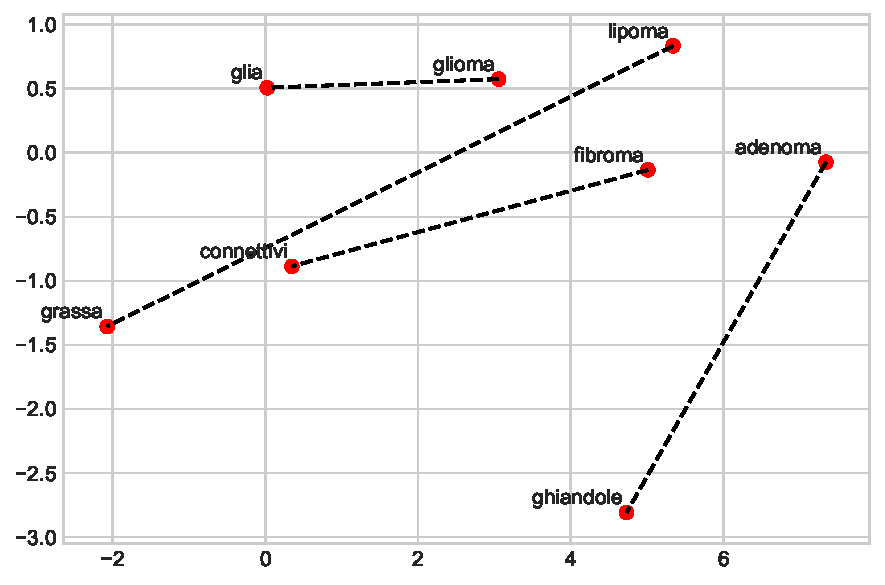
\includegraphics[width=0.5\textwidth]{img/gloveGraph.pdf}
  \caption{Extract from constructed vector space. The Italian labels
    are \emph{grassa} for \emph{fat}, \emph{connettivi} for
    \emph{connectives}, \emph{ghiandole} for \emph{glands}.}
  \label{fig:gloveGraph}
\end{figure}

Most algorithms for obtaining word vectors are based on co-occurrences
in large text corpora. Co-occurrence can be measured either at the
word-document level (e.g.\ using latent semantic analysis) or at the
word-word level (e.g.\ using word2vec~\cite{mikolov_linguistic_2013}
or \ac{glove}~\cite{pennington_glove:_2014}). It is a common practice to
take advantage of pre-compiled libraries of word vectors trained on
several billion tokens extracted from various sources such as
Wikipedia, the English Gigaword 5, Common Crawl, or Twitter. These
libraries are generally conceived for general purpose applications and
are only available for the English language. Since our cancer registry
textual data is written in Italian and employs a very specific domain
terminology, we retrained word vectors from the almost 1.5 millions
unlabeled records described in Section~\ref{sec:dataset}. For this
purpose, we trained \ac{glove}~\cite{pennington_glove:_2014}. An
excerpt of the trained dataset is visible in \cref{fig:gloveGraph}.

The training process involves the construction of the
$n\times n$ triangular matrix $C$ of words co-occurrence, where $n$ is
the number of unique words $w_1,\dots,w_n$ inside the text (possibly
with the exclusion of the
  most and the least frequent terms). In order to do this, a window of
size $\omega$ slides
through the text. After the construction of $C$, \ac{glove} uses the
information contained in it to train a model that produces vector of
specific dimension $\nu$. $\omega$, $\nu$, and the number of
training iterations $\eta$ are the hyperparameters of the method. 

\section{Attention models}
Conditioned generation with attention is a powerful architecture. They
find the main application in the context of sequence-to-sequence
generation.

The first results with attentive models where due to Bahdanau et al.\
\cite{bahdanau_neural_2014}, who used an architecture based on two
parts. The task of the first part is to encode the input using an
\ac{rnn} to create hidden representations of the sequence. Contrarily
to previous approaches, the sequence is not encoded in a single
representation, but each word of the input have his
representation. The second part generate the output
sequence, with a generative \ac{rnn}, using a weighted average of the
input representation to condition the generation. The weights are
calculated by the attention mechanism, based on the values of the
hidden representation of the input, and the state of the output
generating \ac{rnn}. The attention mechanism is trained together with
the rest of the model. Luong et al.\ \cite{luong2015effective}
explored variation on the attention mechanism leading to some
improvement.

\section{Hierarchical models}
In \cite{yang_hierarchical_2016} and \cite{wang2019multi}

\section{\acs{bert}}
\ac{bert} \cite{devlin2018bert} is a recent model that represents the
state of the art in many \ac{nlp} related tasks
\cite{chatterjee2019semeval,hu2019introductory,lee2019biobert,tshitoyan2019unsupervised}.
It is a
bi-directional pre-training model backboned by the Transformer Encoder
\cite{vaswani2017attention}. It is an attention-based technique that
learns context-dependent word representation on large unlabeled
corpora, and then the model is fine tuned end to end on specific labeled
tasks. During pre-training, the model is trained
on unlabeled data over two different tasks. In \ac{mlm} some tokens
are masked and the model is trained to predict those token based on
the context. In \ac{nsp} the model is trained to understand the
relationship between sentences predicting if two sentences are actually
consecutive or if they where randomly replaced (with 50\%
probability). After the pre-training, the model is fine-tuned to the
specific task.



%%% Local Variables:
%%% mode: latex
%%% TeX-master: "thesis"
%%% End:
